\section{Considerações Iniciais}

A fundamentação teórica deste estudo começa com um Mapeamento Sistemático (MS), cujo objetivo é identificar a interseção entre as TICs e as línguas de sinais no contexto educacional. A \autoref{section:foundation:sm} oferece um resumo deste MS, enquanto análises mais detalhadas dos estudos primários, que abrangem tanto o panorama nacional quanto internacional, estão disponíveis em nossas publicações anteriores \cite{FalvoJr2020_FIE, FalvoJr2020_SBIE, FalvoJr2020_RENOTE}.

A realização deste estudo permitiu identificar \textit{gaps} tecnológicos no uso de línguas de sinais no ensino-aprendizagem, destacando a necessidade de novas pesquisas na literatura. Complementar ao MS, um levantamento bibliográfico complementar foi conduzido para explorar conceitos e TICs promissoras que possam enfrentar esses desafios. As seções subsequentes expandem essas temáticas, abordando Arquiteturas de Software (\autoref{section:foundation:arch}), OAs (\autoref{section:foundation:lo}) e ASR (\autoref{section:foundation:asr}). Fornecendo assim, a base teórica para a \textit{Speech2Learning}, uma arquitetura baseada em ASR para OAs audíveis mais acessíveis, definida em detalhes no \autoref{chapter3}.

\section{Mapeamento Sistemático: TICs e Línguas de Sinais no Processo de Ensino-Aprendizagem}
\label{section:foundation:sm}

Para definir o escopo deste projeto, foi crucial realizar um estudo sistemático de literatura para identificar lacunas e oportunidades tecnológicas no processo de ensino e aprendizagem com línguas de sinais. De acordo com \citeonline{Kitchenham2007}, existem duas abordagens principais para este tipo de estudo: Revisão Sistemática (RS) e MS. Optou-se pelo MS devido à sua capacidade de apresentar evidências de um domínio de estudo em um alto nível de granularidade, agrupando-as em áreas de similaridade e identificando tendências emergentes.

O protocolo de pesquisa para o MS foi cuidadosamente definido com base em diretrizes formais  \cite{Kitchenham2007, Zhang2011, Petersen2015}. A abordagem de \citeonline{Zhang2011} foi particularmente relevante, pois orientou a estratégia de busca e os critérios de qualidade adotados no estudo. Essa estratégia foi adaptada para aumentar o rigor do processo de pesquisa, incorporando o \textit{Quasi-Gold Standard} (QGS) e seguindo boas práticas recomendadas na literatura (\autoref{ms:zhang-approach}).

\begin{figure}[htbp]
\caption{Busca sistemática baseada em QGS.}
\label{ms:zhang-approach}
\centerline{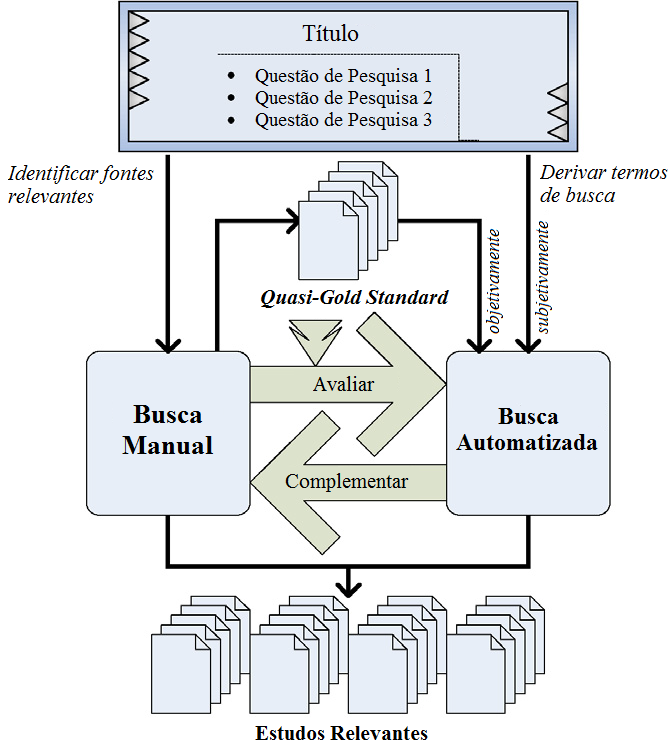
\includegraphics[width=0.5\textwidth]{images/zhang-systematic-mapping-approach.png}}
\caption*{Fonte: Adaptada de \cite{Zhang2011}.}
\end{figure}

\subsection{Definição do Escopo e Critérios de Seleção}
\label{ms:conducao-escopo}

As Questões de Pesquisa (QP) são essenciais para definir o escopo e identificar possíveis palavras-chave em um estudo sistemático de literatura \cite{Kitchenham2007,Petersen2015}. Neste contexto, uma abordagem comum se dá através da aplicação dos critérios de PICO \cite{Petticrew2008}. A \autoref{table:pico} representa o PICO, seguida pelas QP que definem o escopo deste MS.

\begin{table}[!ht]
\caption{Critérios de PICO.}
\label{table:pico}
\centering
\begin{tabular}{ll}
\toprule
\textit{\textbf{P}opulation} & Aprendizes/Educadores interessados em línguas de sinais. \\
\textit{\textbf{I}ntervention} & TICs relevantes no processo de ensino-aprendizagem com línguas de sinais. \\
\textit{\textbf{C}omparison} & Não se aplica. \\
\textit{\textbf{O}utcome} & Panorama tecnológico sobre o ensino-aprendizagem com línguas de sinais. \\ 
\bottomrule
\end{tabular}
\end{table}

\begin{itemize}
    \setlength\itemsep{0em}
    \item \textbf{QP1}: Quais soluções tecnológicas vêm sendo propostas para o ensino e aprendizagem por meio das línguas de sinais?
    % \begin{itemize}
    %     \item Quais são os tipos de soluções propostas (software ou hardware ou teóricas)?
    %     \item Quais tecnologias foram usadas?
    %     \item Quais métodos de avaliação foram aplicados?
    % \end{itemize}
    \item \textbf{QP2}: Quais tópicos educacionais são abordados?
    \item \textbf{QP3}: Quais línguas de sinais são abordadas?
    % \begin{itemize}
    %     \item Quais estudos abordam múltiplas línguas de sinais?
    % \end{itemize}
\end{itemize}

Segundo \citeonline{Kitchenham2007,Petersen2015}, os estudos sistemáticos requerem critérios explícitos de inclusão e exclusão para avaliar seus potenciais estudos primários. Assim, foram definimos os seguintes critérios de seleção:

\begin{table}[htbp]
\caption{Critérios de Inclusão (CI) e Exclusão (CE).}
\label{tab:ms:criterios-selecao}
\centering
\begin{tabularx}{\textwidth}{C{1cm}|X} \hline
\textbf{CI1} & Os estudos apresentam contribuições (software ou hardware ou teóricas) para o ensino e a aprendizagem de línguas de sinais. \\ \hline
\textbf{CE1} & Estudos que não foram publicados no período de 2000 a 2019, seguindo um racional semelhante à \citeonline{Radermacher2013,Scatalon2019}, os quais sugerem que estudos anteriores a 2000 não representam as abordagens educacionais atuais, especialmente considerando o contexto de tecnologia. \\ \hline
\textbf{CE2} & Estudos classificados como resumos, resumos de conferências/editoriais, literatura cinza ou capítulos de livros. \\ \hline
\textbf{CE3} & Estudos não apresentados em inglês ou português. \\ \hline
\textbf{CE4} & Estudos não acessíveis em texto completo. \\ \hline
\textbf{CE5} & Estudos duplicados ou superficialmente complementares de outros estudos. \\ \hline
\end{tabularx}
\end{table}

\subsection{Busca Manual}
\label{ms:conducao-busca-manual}

A \autoref{ms:table:busca-manual-nacional} lista as conferências e periódicos nacionais analisados durante a busca manual. No entanto, os estudos dessas fontes não foram incluídos na composição do QGS devido à limitação de indexação nos mecanismos de busca internacionais, o que poderia comprometer a eficácia da abordagem sistemática baseada em QGS \cite{Zhang2011}. Apesar disso, 46 estudos primários de fontes brasileiras foram considerados e discutidos nos resultados deste MS. Já a \autoref{ms:table:busca-manual-internacional} apresenta as conferências e periódicos internacionais selecionados durante a busca manual, resultando em 19 estudos primários que compõem o QGS deste MS. As fontes relevantes foram utilizadas para a busca automatizada, garantindo uma sinergia maior com o QGS, conforme recomendado por \citeonline{Zhang2011}.

\begin{table}[htbp]
\caption{Busca manual nacional.}
\label{ms:table:busca-manual-nacional}
\centering
\begin{tabular}{lcc}
\hline
\textbf{Conferências/Periódicos} & \textbf{Fonte} & \textbf{Selecionados} \\ \hline
DesafIE                          & CEIE           & -                     \\
JAIE                             & CEIE           & -                     \\
RBIE                             & CEIE           & 2                     \\
RENOTE                           & CINTED         & 13                    \\
SBIE                             & CEIE           & 13                    \\
WAVE2                            & CEIE           & -                     \\
WCBIE                            & CEIE           & 11                    \\
WIE                              & CEIE           & 7                     \\
\multicolumn{2}{l}{\textbf{Total}}                & \textbf{46}           \\ \hline
\end{tabular}
\end{table}

\begin{table}[htbp]
\centering
\caption{Busca manual internacional (QGS).}
\label{ms:table:busca-manual-internacional}
\begin{tabular}{lcc}
\hline
\textbf{Conferência/Periódico} & \textbf{Fonte}     & \textbf{Selecionados (QGS)} \\ \hline
ACM TOCE                       & ACM                & 0            \\ 
Computers \& Education         & Elsevier           & 5            \\ 
FIE                            & IEEE               & 0            \\ 
HCI International              & Springer           & 5            \\ 
ICALT                          & IEEE               & 5            \\ 
IEEE Trans. Educ.              & IEEE               & 1            \\ 
IEEE Trans. Learn. Technol.    & IEEE               & 0            \\ 
Informatics in Education       & Vilnius University & 0            \\ 
ITiCSE                         & ACM                & 2            \\ 
Learning @ Scale               & ACM                & 0            \\ 
SIGCSE                         & ACM                & 1            \\ 
\textbf{Total}                 & \textbf{}          & \textbf{19}  \\ \hline
\end{tabular}
\end{table}


\subsection{Busca Automatizada}
\label{ms:conducao-busca-automatizada}

Duas estratégias para identificação de palavras-chave foram utilizadas em conjunto para nossa string de busca: (i) análise do PICO e suas respectivas QP; (ii) importação da tripla \textit{title-abstract-keywords} em um software de análise de frequência. Os resultados desse processo produziram a seguinte string de busca:

\begin{center}
    (\textit{learn} \textbf{OR} \textit{learning} \textbf{OR} \textit{teach} \textbf{OR} \textit{teaching}) \textbf{AND}\\
    (``\textit{sign language}'' \textbf{OR} ``\textit{signed language}'') \textbf{AND}\\
    (\textit{technology} \textbf{OR} \textit{technologies})\\
\end{center}

A \autoref{method:table:automated-search} resume os resultados da busca automatizada, onde a seleção dos estudos seguiu o mesmo racional apresentado na busca manual. Além disso, a busca automatizada retornou a maioria dos estudos selecionados pela busca manual (QGS), o que sugere uma boa sensibilidade da string de busca. Nesse sentido, \citeonline{Zhang2011} propõem o conceito de \textit{quasi-sensibility}, uma derivação da sensibilidade tradicional que incorpora o QGS como critério de qualidade (\autoref{method:equation:quasi-sensitivity}).

\begin{table}[htbp]
\centering
\caption{Resultados da busca automatizada.}
\label{method:table:automated-search}
\begin{tabular}{lllll}
\hline
 &  & Busca Final &                 &                   \\ \cline{3-5} 
Base de Dados & \textbf{QGS} & Recuperados    & \textbf{no QGS} & \textbf{Relevantes} \\ \hline
ACM DigitalLibrary & 3            & 922          & 3               & 47                \\
IEEE Xplore        & 6            & 359          & 5               & 59                \\
ScienceDirect      & 5            & 1,961        & 5               & 20                \\
SpringerLink       & 5            & 4,980        & 5               & 36                \\
\textbf{Total}   & \textbf{19}  & 8,222        & \textbf{18}     & \textbf{162}      \\ \hline
\end{tabular}
\end{table}

\begin{equation}
\label{method:equation:quasi-sensitivity}
\text{\textit{quasi-sensibility}} = \frac{\text{\textit{Estudos relevantes recuperados (\textbf{no QGS})}}}{\text{\textit{Total de estudos relevantes (\textbf{QGS})}}}
\end{equation}

Como resultado, a \textit{quasi-sensitivity} calculada foi 94,74\% (18/19). Segundo \citeonline{Zhang2011}, esse desempenho da pesquisa é adequado. Portanto, os 163 artigos selecionados pelas buscas (manual e automatizada) foram considerados estudos primários em potencial. Nesta etapa, 24 estudos foram excluídos de acordo com os critérios de inclusão e exclusão pré-estabelecidos. A \autoref{method:figure:evaluation-refinement} organiza os 139 estudos primários, tendo em vista a abordagem de busca sistemática baseada em QGS.

\begin{figure}[htbp]
\caption{Resultados da busca sistemática baseada em QGS.}
\label{method:figure:evaluation-refinement}
\centerline{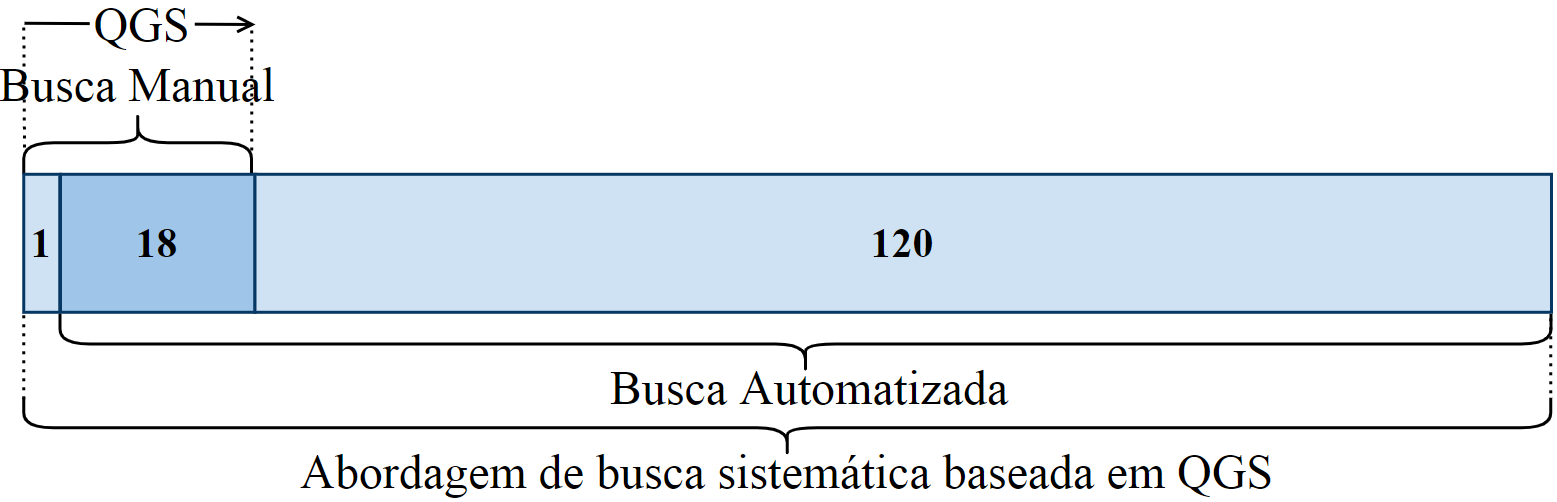
\includegraphics[width=0.85\textwidth]{images/systematic-mapping.png}}
\end{figure}

\subsection{Extração de Dados}
\label{ms:conducao-extracao-dados}

Para extrair as informações relevantes dos estudos primários identificados, um formulário de extração de dados foi criado. A \autoref{method:table:data-extraction} representa o modelo que descreve as informações extraídas e apresenta seu relacionamento com cada QP, quando aplicável.

\begin{table}[htbp]
\centering
\caption{Formulário de extração de dados.}
\label{method:table:data-extraction}
\begin{tabular}{lll}
\hline
\textbf{Item} & \textbf{Descrição} & \textbf{QP} \\ \hline
\textit{\textbf{Informações Gerais}} & & \\ \hline
ID & Identificador (prefixos \textit{INT} ou \textit{BRA}). & \\
Título & Título do estudo. & \\
Autores & Nomes dos autores. & \\
Ano & Ano de publicação do artigo. & \\
Conferência/Periódico & Nome do meio de publicação. & \\
Tipo de busca & Manual; Automatizada; Ambas. & \\
Língua & Inglês; Português. & \\
País & País da afiliação do primeiro autor. & \\ \hline
\textit{\textbf{Informações Específicas}} & & \\ \hline
Área da ES & Área de conhecimento da ES (SWEBOK). & QP1 \\
Tipo de solução & Software; Hardware; Teórica. & QP1 \\
Estratégia empírica & Quais estratégias empíricas foram encontradas. & QP1 \\
Tópico educacional & Quais tópicos educacionais foram encontrados. & QP2 \\
Línguas de sinais & Quais línguas de sinais foram encontradas. & QP3 \\ \hline
\end{tabular}
\end{table}

\subsection{Resultados e Discussões}
\label{ms:resultados}

Considerando os 185 estudos primários selecionados pelo MS, as informações mais relevantes para as QP foram sintetizadas seguindo a estrutura do formulário de extração de dados. Primeiramente, considerando a quantidade de publicações por ano, uma linha de tendência linear crescente foi identificada (\autoref{results:figure:publications-year}). Portanto, é estatisticamente possível que este domínio de pesquisa esteja em ascensão globalmente.

\begin{figure}[htbp]
\caption{Linha de tendência linear ($R^2$) de publicações por ano.}
\label{results:figure:publications-year}
\centerline{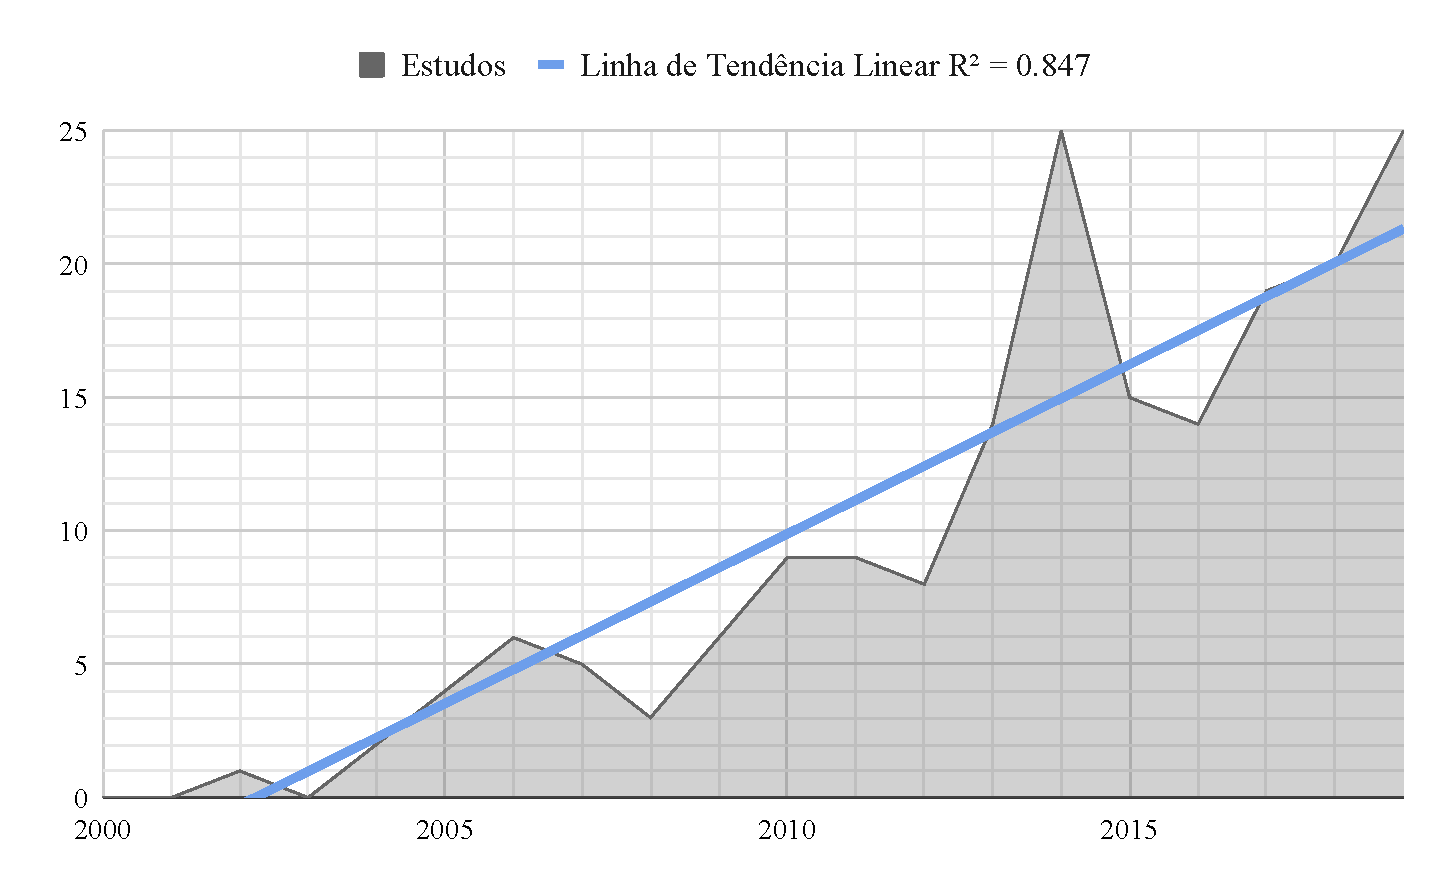
\includegraphics[width=1\textwidth]{images/publications-sm-timeline.pdf}}
\end{figure}

No que diz respeito às fontes das publicações, que também podem compor o racional das buscas manuais em possíveis estudos futuros. A \autoref{results:table:publication-venues} apresenta os principais locais de publicação, considerando todos os estudos primários deste MS, os quais estão ordenados pela quantidade de estudos selecionados. No contexto internacional, a presença de conferências e periódicos definidos na busca manual (em destaque na \autoref{results:table:publication-venues}) sugere uma execução efetiva dessa fase considerando o protocolo de busca adotado.

\begin{table}[htbp]
\caption{Conferências/Periódicos mais relevantes.}
\label{results:table:publication-venues}
\centering
\begin{tabular}{lcc|lcc}
\hline
\multicolumn{3}{c|}{\textbf{Internacionais (\textit{INT})}} & \multicolumn{3}{c}{\textbf{Nacionais (\textit{BRA})}} \\ \hline
\textbf{Nome} & \textbf{Fonte} & \textbf{Estudos} & \textbf{Nome} & \textbf{Fonte} & \textbf{Estudos} \\ \hline
\textit{\textbf{HCI International}} & \textit{\textbf{Springer}} & \textit{\textbf{12}} & RENOTE & CINTED & 13 \\ 
ICCHP & Springer & 8 & SBIE & CEIE & 13 \\ 
\textit{\textbf{ICALT}} & \textit{\textbf{IEEE}} & \textit{\textbf{6}} & WCBIE & CEIE & 11 \\ 
ASSETS & ACM & 6 & WIE & CEIE & 7 \\ 
\textit{\textbf{Computers \& Education}} & \textit{\textbf{Elsevier}} & \textit{\textbf{5}} & RBIE & CEIE & 2 \\ 
Procedia Computer Science & Elsevier & 5 & - & - & - \\ 
Outros & - & 97 & - & - & - \\ 
\multicolumn{2}{l}{\textbf{Total}} & \textbf{139} & \multicolumn{2}{l}{\textbf{Total}} & \textbf{46} \\ \hline
\end{tabular}
\end{table}

A seguir são discutidos os principais resultados deste estudo, de modo a responder cada QP definida no escopo do MS. Adicionalmente, com o objetivo de organizar os estudos primários, eles foram classificados com relação à sua origem: Internacional (\textit{INT})\footnote{Formulário de extração de dados Internacionais (INT): \url{https://bit.ly/SM-DataExtraction-INT}} ou Nacional (\textit{BRA})\footnote{Formulário de extração de dados Nacionais (BRA): \url{https://bit.ly/SM-DataExtraction-BRA}}. Com isso, os resultados podem ser analisados de forma isolada, o que facilita o planejamento e a condução de trabalhos futuros.

\begin{itemize}

\item \textbf{QP1: Quais soluções tecnológicas vêm sendo propostas para o ensino e aprendizagem por meio das línguas de sinais?}

A análise apresentada na \autoref{results:table:se-areas} destaca a importância das Arquiteturas de Software no desenvolvimento de soluções tecnológicas para o ensino e a aprendizagem com línguas de sinais. Embora haja uma ênfase significativa nas etapas de ``Construção'' e ``Projeto'', poucas soluções se mostraram realmente replicáveis e adaptáveis a diferentes contextos educacionais. 

Em contrapartida, avatares de línguas de sinais baseados em texto, como o \textit{Hand Talk}\footnote{Disponível em \url{https://handtalk.me}} e o \textit{VLibras}\footnote{Disponível em \url{https://gov.br/governodigital/pt-br/vlibras}}, destacam-se ao transformar texto em língua de sinais, evidenciando o potencial de projetos bem estruturados na acessibilidade de conteúdos em diversos contextos educacionais. Portanto, a discussão sobre Arquiteturas de Software na \autoref{section:foundation:arch} será fundamental para compreender como essas soluções podem ser aprimoradas para desenvolver tecnologias assistivas verdadeiramente escaláveis.

\begin{table}[htbp]
\caption{QP1: Áreas da ES, conforme o SWEBOK \cite{Bourque2014}.}
\label{results:table:se-areas}
\centering
\begin{tabular}{lcccc}
\hline
 & \multicolumn{2}{c}{\textit{\textbf{INT}}} & \multicolumn{2}{c}{\textit{\textbf{BRA}}} \\ \cline{2-5} 
\textbf{Área da ES} & \textbf{Estudos} & \textbf{\%} & \textbf{Estudos} & \textbf{\%} \\ \hline
Construção de Software & 65 & 47\% & 23 & 50\% \\
Projeto de Software & 47 & 34\% & 5 & 11\% \\
Fundamentos da Engenharia & 24 & 17\% & 9 & 19\% \\
Qualidade de Software & 3 & 2\% & 9 & 19\% \\
\textbf{Total} & \textbf{139} & \textbf{100\%} & \textbf{46} & \textbf{100\%} \\ \hline
\end{tabular}
\end{table}

\item \textbf{QP2: Quais tópicos educacionais são abordados?}

A \autoref{results:table:educational-topics} revela uma ampla diversidade de tópicos educacionais nos OAs analisados, evidenciando o uso de tecnologias assistivas para línguas de sinais em diversos contextos. O que representa um esforço consciente em abordar diferentes temas no processo de ensino-aprendizagem, promovendo uma acessibilidade digital mais ampla e personalizada. 

Com uma vasta gama de OAs inclusivos e adaptáveis, os educadores podem proporcionar experiências de aprendizado mais imersivas e eficazes, garantindo oportunidades igualitárias de desenvolvimento para todos os alunos, independentemente de suas habilidades ou desafios individuais. Esses resultados estabelecem a base para uma discussão mais aprofundada sobre OAs na \autoref{section:foundation:lo}, onde exploraremos como esses recursos podem ser projetados para atender demandas educacionais diversas.

\begin{table}[htbp]
\caption{QP2: Tópicos Educacionais.}
\label{results:table:educational-topics}
\centering
\begin{tabular}{lcccc}
\hline
 & \multicolumn{2}{c}{\textit{\textbf{INT}}} & \multicolumn{2}{c}{\textit{\textbf{BRA}}} \\ \cline{2-5} 
\textbf{Tópico Educacional} & \textbf{Estudos} & \textbf{\%} & \textbf{Estudos} & \textbf{\%} \\ \hline
Línguas de Sinais & 59 & 42,5\% & 19 & 41,3\% \\
Geral & 48 & 34,5\% & 10 & 21,7\% \\
Língua de Sinais Escrita & 10 & 7,2\% & 3 & 6,5\% \\
Matemática & 7 & 5,0\% & - & - \\
Alfabeto & 6 & 4,3\% & 1 & 2,2\% \\
Ciência da Computação & 4 & 2,9\% & 4 & 8,7\% \\
Língua Falada do País & 2 & 1,4\% & 9 & 19,6\% \\
Outros & 3 & 2,2\% & - & - \\
\textbf{Total} & \textbf{139} & \textbf{100\%} & \textbf{46} & \textbf{100\%} \\ \hline
\end{tabular}
\end{table}

\item \textbf{QP3: Quais línguas de sinais são abordadas?}

A \autoref{results:table:sign-languages} evidencia uma concentração em línguas de sinais específicas, que, aliada ao crescente interesse pelo conceito de ASR multilíngue, aponta para novas fronteiras na promoção da acessibilidade. Nesse sentido, o uso de IAs Generativas (IAGen) para transcrever e traduzir fala em texto em diferentes línguas faladas oferece um mecanismo poderoso para integrar avatares de línguas de sinais baseados em texto, permitindo a criação de OAs mais inclusivos e flexíveis.

Nesse contexto, línguas de sinais como ASL, Libras, ArSL e sistemas de escrita como SignWriting podem se beneficiar significativamente dessas tecnologias, permitindo um acesso mais amplo e facilitado a conteúdos educacionais anteriormente disponíveis apenas em formato áudio. Esses achados introduzem o tema do Reconhecimento Automático de Fala, que será detalhado na \autoref{section:foundation:asr}, com foco em como o ASR pode ser utilizado para melhorar a acessibilidade e a qualidade dos conteúdos educacionais.

\begin{table}[htbp]
\caption{QP3: Línguas de Sinais.}
\label{results:table:sign-languages}
\centering
\begin{tabular}{lcccc}
\hline
 & \multicolumn{2}{c}{\textit{\textbf{INT}}} & \multicolumn{2}{c}{\textit{\textbf{BRA}}} \\ \cline{2-5} 
\textbf{Língua de Sinais} & \textbf{Estudos} & \textbf{\%} & \textbf{Estudo} & \textbf{\%} \\ \hline
ASL & 21 & 15.11\% & - & - \\
Libras & 16 & 11.51\% & 44 & 95.65\% \\
Geral & 15 & 10.79\% & - & - \\
SignWriting & 10 & 7.19\% & 2 & 4.35\% \\
ArSL & 10 & 7.19\% & - & - \\
PSL & 6 & 4.32\% & - & - \\
BSL & 6 & 4.32\% & - & - \\
MySL & 6 & 4.32\% & - & - \\
ISL & 5 & 3.60\% & - & - \\
Outras & 44 & 31.65\% & - & - \\
\textbf{Total} & \textbf{139} & \textbf{100\%} & \textbf{46} & \textbf{100\%} \\ \hline
\end{tabular}
\end{table}

\end{itemize}

A análise dos resultados obtidos das QPs fornece um panorama do uso das TICs no ensino e aprendizado com línguas de sinais, revelando tanto lacunas quanto oportunidades para avanços futuros. Essas descobertas abrem caminho para uma exploração detalhada de temas cruciais, como Arquiteturas de Software (\autoref{section:foundation:arch}), OAs (\autoref{section:foundation:lo}) e ASR (\autoref{section:foundation:asr}). 

Cada seção subsequente destaca como suas temáticas podem ajudar a superar os desafios identificados e a capitalizar nas oportunidades emergentes, contribuindo para um processo de ensino-aprendizagem mais inclusivo e acessível.

\section{Arquiteturas de Software: Bases Sólidas para Tecnologias Assistivas}
\label{section:foundation:arch}

Uma das principais lacunas identificadas no MS foi a falta de padrões e boas práticas que permitam o reuso e a adaptação das soluções para o ensino e aprendizagem com línguas de sinais. Muitos dos estudos primários apresentaram tecnologias assistivas relevantes, mas não detalharam as arquiteturas de software utilizadas, dificultando a replicação e a extensão dessas soluções para outros contextos e domínios de aplicação. Por isso, discutiremos como as arquiteturas podem contribuir para o desenvolvimento de projetos replicáveis, flexíveis e independentes de tecnologia, seguindo alguns princípios e diretrizes da engenharia de software.

Tecnicamente, uma arquitetura de software é a estrutura fundamental de uma solução, que define os componentes, as interfaces, as responsabilidades, as dependências, entre outras propriedades do sistema \cite{Bass2021}. A escolha de uma arquitetura adequada é fundamental para garantir a qualidade, a manutenibilidade, a escalabilidade e a portabilidade de um software. Além disso, quando bem definida e documentada, facilita a comunicação entre os desenvolvedores, os usuários e os \textit{stakeholders} do sistema, bem como a reutilização de componentes e boas práticas em outros projetos \cite{Sommerville2015, Pressman2016}.

\section{Objetos de Aprendizagem: Diversidade em Conteúdos Educacionais}
\label{section:foundation:lo}

Os Objetos de Aprendizagem (OAs) representam um espectro amplo de recursos digitais, estrategicamente projetados para suportar o processo educacional. Eles são essenciais para transcender a tradicional entrega de conteúdo, possibilitando uma experiência de aprendizagem mais rica e interativa. \citeonline{Mayer2021} destacam a importância da multimídia no aprendizado, argumentando que a combinação eficaz de texto, áudio, vídeo e visualizações interativas pode significativamente melhorar a retenção e a aplicação do conhecimento por parte dos alunos.

A inclusão de transcrições em materiais audíveis, como videoaulas, exemplifica a flexibilidade e expansividade dos OAs. Esta prática não apenas facilita o acesso à informação para todos os alunos, mas também destaca o potencial dos OAs em adaptar-se às necessidades de uma gama diversificada de aprendizes, promovendo uma educação mais inclusiva. Esta capacidade de adaptação dos OAs sinaliza para a importância de tecnologias emergentes, como o reconhecimento de fala, em ampliar ainda mais a acessibilidade e personalização dos conteúdos educacionais.

\section{Reconhecimento de Fala: Promovendo Acessibilidade Digital com IA}
\label{section:foundation:asr}

Na era digital, a educação está em constante evolução à medida que as tecnologias emergentes podem remodelar as abordagens pedagógicas tradicionais. Neste contexto, o ASR, interpretado neste trabalho como um sinônimo de STT, emerge como uma ferramenta poderosa. O conceito de ASR não apenas pode potencializar a acessibilidade de conteúdos com transcrições e legendas, mas também representa um passo significativo em direção a uma educação mais inclusiva. Nesse sentido, concordamos com \citeonline{homburg2019} sobre o potencial do ASR nas tecnologias assistivas para surdos, dentre as quais destacamos os avatares de línguas de sinais baseados em texto em nosso MS \cite{FalvoJr2020_SBIE, FalvoJr2020_FIE, FalvoJr2020_RENOTE}.

Segundo \citeonline{fleischmann2021}, a ascensão do ensino remoto, acelerada por circunstâncias como a pandemia da COVID-19, impulsionou a busca por métodos inovadores para a criação e compartilhamento de conteúdos educacionais. Nessa conjuntura, o ASR se consolidou como uma ferramenta promissora, particularmente em ambientes colaborativos ou conferências online. 

Desta forma, soluções baseadas em ASR desempenham um papel vital ao quebrar barreiras linguísticas, otimizando a comunicação entre falantes de diferentes línguas. Este argumento e reforçado por \citeonline{homburg2019}, que destaca a relevância da tradução de voz para línguas de sinais visando promover a inclusão da comunidade surda no processo de ensino-aprendizagem.

Apesar de seu potencial, o ASR enfrenta diversos obstáculos e desafios de pesquisa. O trabalho de \citeonline{koenecke2020} destaca alguns deles, apontando para disparidades raciais e as sutilezas de características linguísticas, como sotaques e peculiaridades regionais, assim como identificamos em nosso MS para a Libras. Essas constatações reforçam a relevância de promover soluções baseadas em ASR que sejam verdadeiramente inclusivas e que contemplem um espectro mais amplo de considerações sociolinguísticas em seu projeto e implementação.

\citeonline{Mayer2021} afirmam que o uso de tecnologias disruptivas, como o ASR, é fundamental para ampliar o alcance dos OAs a uma diversidade maior de aprendizes, promovendo conteúdos educacionais mais acessível. Na prática, \citeonline{parakh2022} descreve OAs como unidades digitais reutilizáveis que muitas vezes são integradas em iniciativas open-source, desempenhando um papel crucial ao moldar experiências de ensino-aprendizagem adaptáveis, democráticas e contextualizadas.

Estas recentes perspectivas reforçam e expandem nossas percepções obtidas em nosso MS, que enfatizou a importância das inovações tecnológicas no processo de ensino e aprendizagem de línguas de sinais, revelando gaps interessantes. Nesse sentido, notamos a falta de padrões de projeto, além de boas práticas de código e reuso, o que compromete a qualidade, o compartilhamento e o potencial de impacto desses OAs. Diante destas lacunas e das tendências emergentes citadas, projetamos a Arquitetura \textit{Speech2Learning}. Uma abstração que propõem diretrizes de desenvolvimento para a criação de soluções \textit{ASR-based}, promovendo maior acessibilidade de seus OAs, em especial os audíveis.

\section{Considerações Finais}